\documentclass[12pt]{report}
\usepackage[utf8]{inputenc}
\usepackage[russian]{babel}
%\usepackage[14pt]{extsizes}
\usepackage{listings}
\usepackage{amsmath}
\usepackage[justification=centering]{caption}

\lstdefinelanguage{Kotlin}{
  comment=[l]{//},
  commentstyle={\color{gray}\ttfamily},
  emph={delegate, filter, first, firstOrNull, forEach, lazy, map, mapNotNull, println, return@},
  emphstyle={\color{OrangeRed}},
  identifierstyle=\color{black},
  keywords={abstract, actual, as, as?, break, by, class, companion, continue, data, do, dynamic, else, enum, expect, false, final, for, fun, get, if, import, in, interface, internal, is, null, object, override, package, private, public, return, set, super, suspend, this, throw, true, try, typealias, val, var, vararg, when, where, while},
  keywordstyle={\color{blue}\bfseries},
  morecomment=[s]{/*}{*/},
  morestring=[b]",
  morestring=[s]{"""*}{*"""},
  ndkeywords={@Deprecated, @JvmField, @JvmName, @JvmOverloads, @JvmStatic, @JvmSynthetic, Array, Byte, Double, Float, Int, Integer, Iterable, Long, Runnable, Short, String},
  ndkeywordstyle={\color{orange}\bfseries},
  sensitive=true,
  stringstyle={\color{green}\ttfamily},
}

% Для листинга кода:
\lstset{ %
language=Kotlin,                 % выбор языка для подсветки (здесь это С)
basicstyle=\footnotesize\sffamily, % размер и начертание шрифта для подсветки кода
numbers=left,               % где поставить нумерацию строк (слева\справа)
numberstyle=\tiny,           % размер шрифта для номеров строк
stepnumber=1,                   % размер шага между двумя номерами строк
numbersep=5pt,                % как далеко отстоят номера строк от подсвечиваемого кода
showspaces=false,            % показывать или нет пробелы специальными отступами
showstringspaces=false,      % показывать или нет пробелы в строках
showtabs=false,             % показывать или нет табуляцию в строках
frame=single,              % рисовать рамку вокруг кода
tabsize=2,                 % размер табуляции по умолчанию равен 2 пробелам
captionpos=t,              % позиция заголовка вверху [t] или внизу [b] 
breaklines=true,           % автоматически переносить строки (да\нет)
breakatwhitespace=false, % переносить строки только если есть пробел
escapeinside={\#*}{*)}   % если нужно добавить комментарии в коде
}

\usepackage{hyperref}
\hypersetup{
    linktoc=all,     %set to all if you want both sections and subsections linked
    linkcolor=blue,  %choose some color if you want links to stand out
}

% Для измененных титулов глав:
\usepackage{titlesec, blindtext, color} % подключаем нужные пакеты
\definecolor{gray75}{gray}{0.75} % определяем цвет
\newcommand{\hsp}{\hspace{20pt}} % длина линии в 20pt
% titleformat определяет стиль
\titleformat{\chapter}[hang]{\Huge\bfseries}{\thechapter\hsp\textcolor{gray75}{|}\hsp}{0pt}{\Huge\bfseries}

% plot
\usepackage{pgfplots}
\usepackage{filecontents}
\usetikzlibrary{datavisualization}
\usetikzlibrary{datavisualization.formats.functions}

\begin{filecontents}{SBSorted.dat}
100 1818544
200 2182084
300 2836575
400 3666706
500 4561938
1000 12282615
1500 25296835
2000 43069012
3000 91881622
4000 165458964
5000 248940636
\end{filecontents}

\begin{filecontents}{SBSortedReverse.dat}
100 1902381
200 2690147
300 3973067
400 6108805
500 8344909
1000 28119897
1500 59508253
2000 102249552
3000 218854972
4000 379629421
5000 592686305
\end{filecontents}

\begin{filecontents}{SBUnsorted.dat}
100 1592950
200 2200640
300 3280409
400 4728961
500 6573267
1000 21195842
1500 45146080
2000 79173129 
3000 166840980
4000 280142359
5000 449032194
\end{filecontents}

\begin{filecontents}{SISorted.dat}
100 1630961
200 1647635
300 1640207
400 1640022
500 1645407
1000 1654109
1500 1662390
2000 1700609
3000 1810398
4000 1823571
5000 1766772
\end{filecontents}

\begin{filecontents}{SISortedReverse.dat}
100 1770645
200 2035881
300 2809635
400 3078558
500 3876786
1000 10741734
1500 21659401
2000 37367527
3000 78513340
4000 131840967
5000 197947307
\end{filecontents}

\begin{filecontents}{SIUnsorted.dat}
100 1498909
200 1562519
300 1808384
400 2184299
500 2566161
1000 5769483
1500 11233626
2000 18556919
3000 38942468
4000 66181509
5000 99391239
\end{filecontents}

\begin{filecontents}{SSSorted.dat}
100 1826308
200 2144446
300 2530081
400 2924786
500 3594866
1000 8634889
1500 17374004
2000 29104145
3000 61997393
4000 105764286
5000 164210924
\end{filecontents}

\begin{filecontents}{SSSortedReverse.dat}
100 1712426
200 1948340
300 2299634
400 2837866
500 3483199
1000 9179446
1500 17961391
2000 30242327
3000 65218978
4000 114500414
5000 173933001
\end{filecontents}

\begin{filecontents}{SSUnsorted.dat}
100 1460379
200 1680307
300 2038358
400 2558087
500 3166091
1000 8411547
1500 17161009
2000 28673064
3000 64444295
4000 102043152
5000 172713187
\end{filecontents}

\begin{document}
\begin{titlepage}
	\fontsize{12pt}{12pt}\selectfont
	\noindent \begin{minipage}{0.15\textwidth}
		
\includegraphics[width=\linewidth]{inc/img/b_logo.jpg}
	\end{minipage}
	\noindent\begin{minipage}{0.9\textwidth}\centering
		\textbf{Министерство науки и высшего образования Российской Федерации}\\
		\textbf{Федеральное государственное бюджетное образовательное учреждение высшего образования}\\
		\textbf{«Московский государственный технический университет имени Н.Э.~Баумана}\\
		\textbf{(национальный исследовательский университет)»}\\
		\textbf{(МГТУ им. Н.Э.~Баумана)}
	\end{minipage}
	
	\noindent\rule{15cm}{3pt}
	\newline\newline
	\noindent ФАКУЛЬТЕТ \underline{~~~~~~~~~~~~~~~~«Информатика и системы управления»~~~~~~~~~~~~~~~~} \newline\newline
	\noindent КАФЕДРА \underline{«Программное обеспечение ЭВМ и информационные технологии»}\newline\newline\newline\newline\newline\newline\newline
	
	
	\begin{center}
		\Large\textbf{Отчет по лабораторной работе №3 по курсу "Анализ алгоритмов"}\newline
	\end{center}
	
	\noindent\textbf{Тема} \underline{Алгоритмы сортировки}\newline\newline\newline
	\noindent\textbf{Студент} \underline{Якуба Д. В.}\newline\newline
	\noindent\textbf{Группа} \underline{ИУ7-53Б}\newline\newline
	\noindent\textbf{Оценка (баллы)} \underline{~~~~~~~~~~~~~~~~~~~}\newline\newline
	\noindent\textbf{Преподаватели} \underline{Волкова Л.Л., Строганов Ю.В.}\newline
	
	\begin{center}
		\vfill
		Москва~---~\the\year
		~г.
	\end{center}
\end{titlepage}

\setcounter{page}{2}

\tableofcontents

\newpage
\chapter*{Введение}
\addcontentsline{toc}{chapter}{Введение}
\section*{Цель лабораторной работы}
Изучение алгоритмов сортировки пузырьком, вставками и выбором.
\section*{Задачи лабораторной работы}
\begin{enumerate}
\item изучение алгоритмов сортировки пузырьком, вставками и выбором;
\item реализация алгоритмов сортировки пузырьком, вставками и выбором;
\item проведение сравнительного анализа трудоёмкости алгоритмов на основе теоретических расчетов и выбранной модели вычислений;
\item сравнительный анализ алгоритмов на основе экспериментальных данных;
\item подготовка отчёта по лабораторной работе;
\item получение практических навыков реализации алгоритмов на ЯП Kotlin.
\end{enumerate}
\section*{Определение}
Сортировка - это процесс перегруппировки заданной последовательности объектов в некотором определённом порядке. Такой определённый порядок позволяет, в некоторых случаях, эффективнее работать с заданной последовательностью.

Пусть требуется упорядочить $N$ элементов: $E_1,E_2,...,E_n$. Каждый элемент представляет из себя запись $E_j$, содержащую некоторую информацию и ключ $K_j$, управляющий процессом сортировки. На множестве ключей определено отношение порядка $<$ так, чтобы для любых трёх значений ключей $a,b,c$ выполнялись следующие условия:

\begin{itemize}
\item Либо $a < b$, либо $b < c$, либо $a = b$;
\item Если $a < b$ и $b < c$, то $a < c$.
\end{itemize}

Данные условия определяют математическое понятие линейного и совершенного упорядочения, а удовлетворяющие им множества поддаются сортировке большинством методов.

Задачей сортировки является нахождение такой перестановки записей $p(1)p(2)...p(n)$ с индексами ${1, 2, ..., N}$, после которой ключи расположились бы в порядке неубывания.

\begin{equation}
K_{p(1)} \leq K_{p(2)} \leq ... \leq K_{p(n)}
\end{equation}

\chapter{Аналитическая часть}

\section{Алгоритм сортировки пузырьком}
Алгоритм заключается в повторяющих проходах по сортируемому массиву. За каждый проход элементы последовательно сравниваются попарно. В том случае, если два элемента расположены не по порядку, то они меняются местами \cite{Knut}. Этот процесс повторяется до тех пор, пока элементы не будут упорядочены, то есть, в случае массива элементов размером $n$, проходы повторятся $n - 1$ раз.

\section{Алгоритм сортировки вставками}
Алгоритм заключается в следующей последовательности действий: элементы просматриваются по одному, и каждый новый элемент вставляется в подходящее место среди ранее упорядоченных элементов \cite{Knut}.

В начальный момент времени отсортированная последовательность пуста. На каждом шаге алгоритма выбирается один из элементов входных данных и помещается на нужную позицию в уже отсортированной последовательности до тех пор, пока набор входных данных не будет исчерпан. В любой момент времени в отсортированной последовательности элементы удовлетворяют требованиям к выходным данным алгоритма.

\section{Алгоритм сортировки выбором}
Алгоритм заключается в следующей последовательности действий: сначала выделяется наименьший (наибольший) элемент последовательности и каким-либо образом отделяется от остальных, затем выбирается наименьший (наибольший) из оставшихся и т.д. \cite{Knut}

\section*{Вывод}
Были рассмотрены алгоритмы сортировки пузырьком, вставками и выбором. В данной работе стоит задача реализации рассмотренных алгоритмов. Также будет необходимо оценить теоретическую оценку алгоритмов и проверить её экспериментально.

\chapter{Конструкторская часть}
\section{Блок-схема алгоритма сортировки пузырьком}
Блок-схема алгоритма сортировки пузырьком предоставлена на рисунке \ref{img:bubbleSortScheme}.

\begin{figure}
\begin{center}
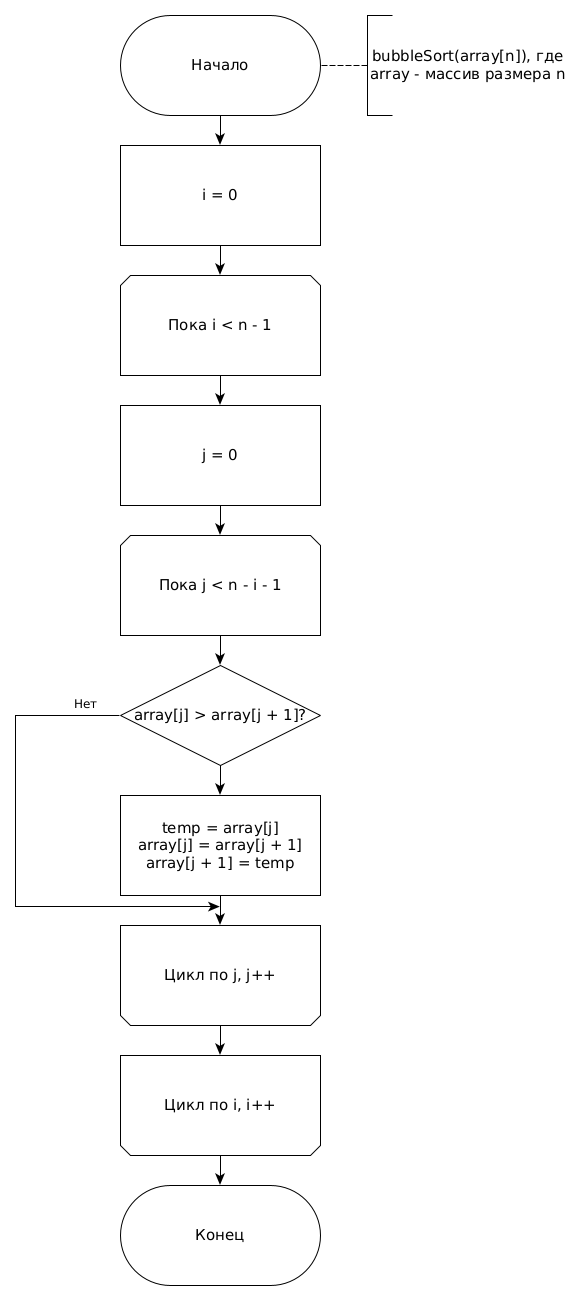
\includegraphics[scale=0.4]{inc/img/bubbleSort.png}
\captionsetup{justification=centering}
	\caption{Блок-схема алгоритма сортировки пузырьком.}
	\label{img:bubbleSortScheme}	
\end{center}
\end{figure}

\section{Блок-схема алгоритма сортировки вставками}
Блок-схема алгоритма сортировки вставками предоставлена на рисунке \ref{img:insertionSortScheme}.

\begin{figure}
\begin{center}
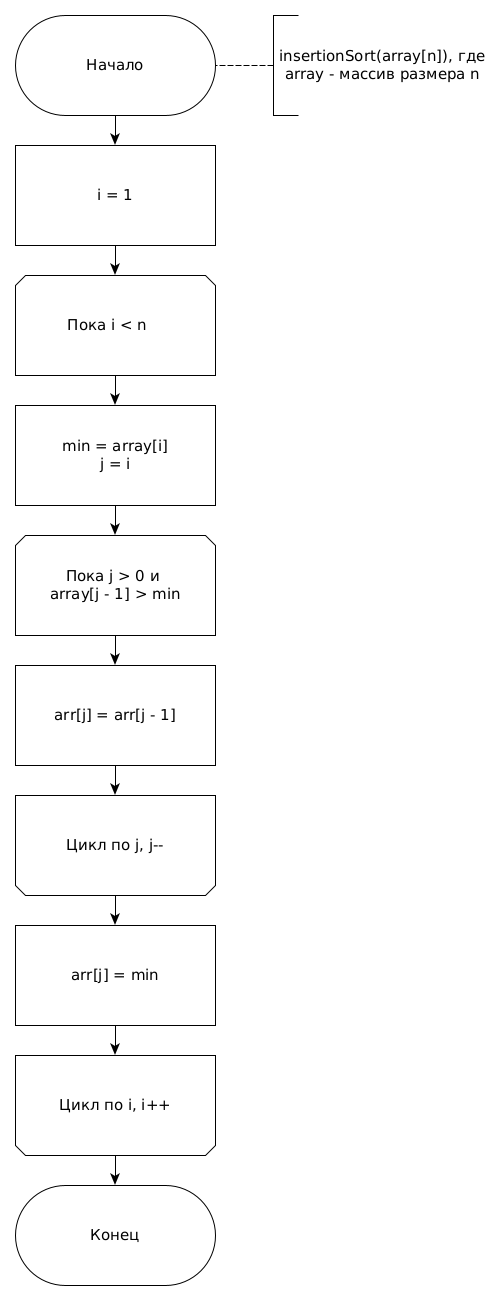
\includegraphics[scale=0.4]{inc/img/insertionSort.png}
\captionsetup{justification=centering}
	\caption{Блок-схема алгоритма сортировки вставками.}
	\label{img:insertionSortScheme}	
\end{center}
\end{figure}

\section{Блок-схема алгоритма сортировки выбором}
Блок-схема алгоритма сортировки выбором предоставлена на рисунке \ref{img:selectionSortScheme}.

\begin{figure}
\begin{center}
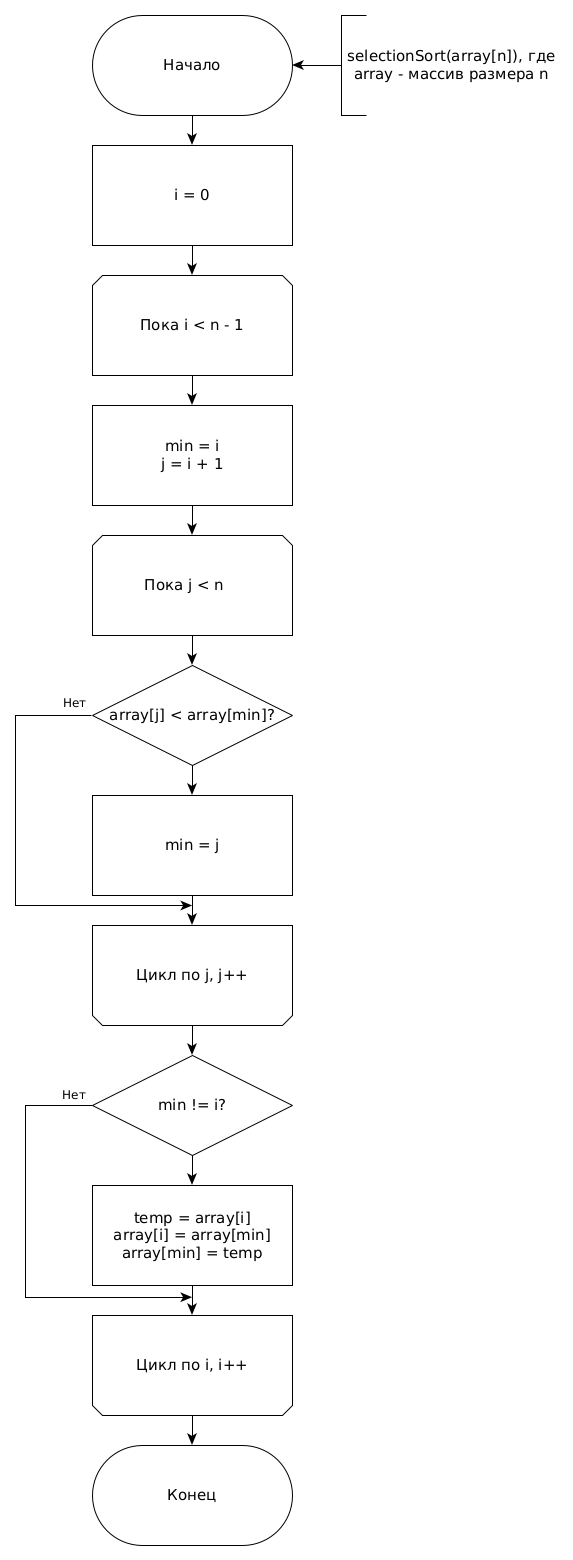
\includegraphics[scale=0.33]{inc/img/selectionSort.png}
\captionsetup{justification=centering}
	\caption{Блок-схема алгоритма сортировки выбором.}
	\label{img:selectionSortScheme}	
\end{center}
\end{figure}

\newpage

\section{Модель вычислений}
ля последующего вычисления трудоемкости необходимо ввести модель вычислений:
\begin{enumerate}
    \item операции из списка (\ref{operators}) имеют трудоемкость 1;
        \begin{equation}
            \label{operators}
            +, -, /, \%, ==, !=, <, >, <=, >=, [], ++, {-}-, +=, -=, *=, \%=
        \end{equation}
    \item трудоемкость оператора выбора \textbf{условие then A else B} рассчитывается, как (\ref{if});
	\begin{equation}
        \label{if}
        f_{if} = f_{\text{условия}} +
        \begin{cases}
        f_A, & \text{если условие выполняется,}\\
        f_B, & \text{иначе.}
        \end{cases}
	\end{equation}
\item трудоемкость цикла рассчитывается, как (\ref{for});
    \begin{equation}
        \label{for}
        f_{for} = f_{\text{инициализации}} + f_{\text{сравнения}} + N(f_{\text{тела}} + f_{\text{инкремента}} + f_{\text{сравнения}})
    \end{equation}
	\item трудоемкость вызова функции равна 0.
\end{enumerate}

\section{Трудоёмкость алгоритмов}
\subsection{Соглашение}
Далее под некоторой величиной $size$ будет подразумеваться длина переданного массива.

\subsection{Алгоритм сортировки пузырьком}
Трудоёмкость алгоритма сортировки пузырьком будет включать включать в себя:
\begin{itemize}
\item цикл по $i \in [0..size - 1]$;
\item цикл по $j \in [0.. size - 1 - i]$, включённый в цикл по i.
\end{itemize}

При этом для цикла по $j$ из части блок-схемы, представленной на рисунке \ref{img:bubble:fj}, будем иметь:

\begin{equation}
f_{j} = 1 + 3 + \frac{1 + (size-1)}{2}(1 + 3 + f_{jbody})
\end{equation}
где $f_{jbody}$ - это трудоёмкость тела цикла, которая определяется выражением:

\begin{equation}
f_{jbody} = 5 + \begin{cases}
				0, & \textbf{лучший случай}\\
				9, & \textbf{худший случай}\\
				\end{cases}
\end{equation}

\begin{figure}
\begin{center}
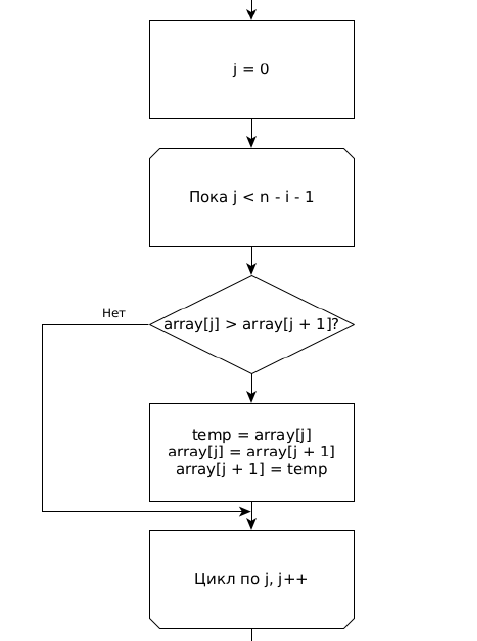
\includegraphics[scale=0.4]{inc/img/bubblefj.png}
\captionsetup{justification=centering}
	\caption{Часть блок-схемы, определяющая $f_{j}$ и $f_{j body}$.}
	\label{img:bubble:fj}	
\end{center}
\end{figure}

Для цикла по $i$ из части блок-схемы, представленной на рисунке \ref{img:bubble:fi}, будем иметь:

\begin{equation}
f_{i} = 1 + 2 + (size - 1)f_{j}
\end{equation}

Как итог, имеем в лучшем случае:
\begin{equation}
f = f_{i} = 3 + (size-1)(4 + \frac{size}{2}(4 + 5)
\end{equation}

\begin{equation}
f = -1 + 4size + \frac{9}{2}{size}^2 - \frac{9}{2}size \approx \frac{9}{2}{size^2} = O({size}^2)
\end{equation}

В худшем случае:
\begin{equation}
f = f_{i} = 3 + (size-1)(4 + \frac{size}{2}(4 + 14)
\end{equation}

\begin{equation}
f = -1 + 4size + 9{size}^2 - 9size \approx 9{size^2} = O({size}^2)
\end{equation}

\begin{figure}
\begin{center}
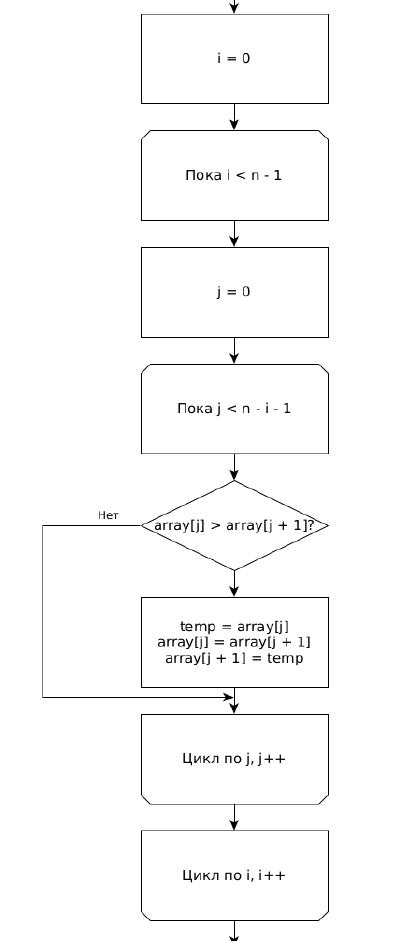
\includegraphics[scale=0.5]{inc/img/bubblefi.png}
\captionsetup{justification=centering}
	\caption{Часть блок-схемы, определяющая $f_{i}$.}
	\label{img:bubble:fi}	
\end{center}
\end{figure}
\newpage 

\subsection{Алгоритм сортировки вставками}
Трудоёмкость алгоритма сортировки вставками будет включать включать в себя:
\begin{itemize}
\item цикл по $i \in [1..size]$;
\item цикл по $j \in [i..0]$, включённый в цикл по i.
\end{itemize}

При этом для цикла по $j$ из части блок-схемы, представленной на рисунке \ref{img:insertion:fj}, будем иметь:

\begin{equation}
f_{j} = 3 + 4 + \frac{size}{2}\begin{cases}
				4, & \textbf{лучший случай}\\
				1 + 4 + f_{jbody}, & \textbf{худший случай}\\
				\end{cases}
\end{equation}
где $f_{jbody}$ - это трудоёмкость тела цикла, которая определяется выражением:

\begin{equation}
f_{jbody} = 4
\end{equation}

\begin{figure}
\begin{center}
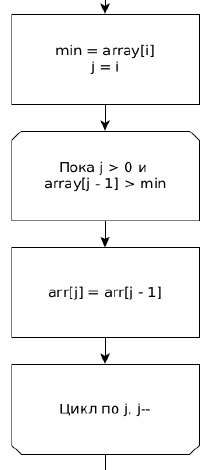
\includegraphics[scale=0.4]{inc/img/insertionfj.png}
\captionsetup{justification=centering}
	\caption{Часть блок-схемы, определяющая $f_{j}$ и $f_{j body}$.}
	\label{img:insertion:fj}	
\end{center}
\end{figure}

Для цикла по $i$ из части блок-схемы, представленной на рисунке \ref{img:insertion:fi}, будем иметь:

\begin{equation}
f_{i} = 1 + 1 + (size - 1)(1 + 1 + f_{j})
\end{equation}

Как итог, имеем в лучшем случае:
\begin{equation}
f = f_{i} = 2 + (size - 1)(9 + 2size)
\end{equation}

\begin{equation}
f = 2{size}^2 + 7size - 7 \approx 2{size}^2 = O({size^2})
\end{equation}

В худшем случае:
\begin{equation}
f = f_{i} = 3 + (size-1)(4 + \frac{size}{2}(4 + 14)
\end{equation}

\begin{equation}
f = -1 + 4size + 9{size}^2 - 9size \approx 9{size^2} = O({size}^2)
\end{equation}

\begin{figure}
\begin{center}
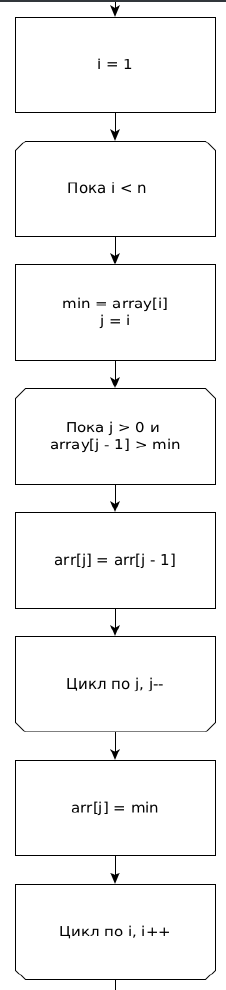
\includegraphics[scale=0.5]{inc/img/insertionfi.png}
\captionsetup{justification=centering}
	\caption{Часть блок-схемы, определяющая $f_{i}$.}вообще
	\label{img:insertion:fi}	
\end{center}
\end{figure}
\newpage 

\subsection{Алгоритм сортировки выбором}
Трудоёмкость алгоритма сортировки выбором будет включать включать в себя:
\begin{itemize}
\item цикл по $i \in [0..size - 1]$;
\item цикл по $j \in [i + 1..size]$, включённый в цикл по i.
\end{itemize}

При этом для цикла по $j$ из части блок-схемы, представленной на рисунке \ref{img:selection:fj}, будем иметь:

\begin{equation}
f_{j} = 3 + 1 + \frac{size}{2}(1 + 1 + f_{jbody})
\end{equation}
где $f_{jbody}$ - это трудоёмкость тела цикла, которая определяется выражением:

\begin{equation}
f_{jbody} = \begin{cases}
				3, & \textbf{лучший случай}\\
				4, & \textbf{худший случай}\\
				\end{cases}
\end{equation}

\begin{figure}
\begin{center}
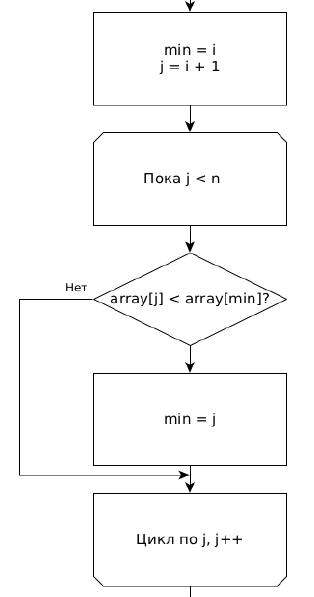
\includegraphics[scale=0.4]{inc/img/selectionfj.png}
\captionsetup{justification=centering}
	\caption{Часть блок-схемы, определяющая $f_{j}$ и $f_{j body}$.}
	\label{img:selection:fj}	
\end{center}
\end{figure}

Для цикла по $i$ из части блок-схемы, представленной на рисунке \ref{img:selection:fi}, будем иметь:

\begin{equation}
f_{i} = 1 + 1 + (size - 1)(1 + 1 + 2 + f_{j})
\end{equation}

Как итог, имеем в лучшем случае:
\begin{equation}
f = f_{i} = 2 + (size - 1)(4 + 4 + \frac{size}{2}(1 + 1 + 3))
\end{equation}

\begin{equation}
f = -6 + \frac{11}{2}size + \frac{5}{2}{size}^2 \approx \frac{5}{2}{size}^2 = O({size}^2)
\end{equation}

В худшем случае:
\begin{equation}
f = f_{i} = 2 + (size - 1)(4 + 4 + \frac{size}{2}(1 + 1 + 4))
\end{equation}

\begin{equation}
f = -6 + 5size + 3{size}^2 \approx 3{size}^2 = O({size}^2)
\end{equation}

\begin{figure}
\begin{center}
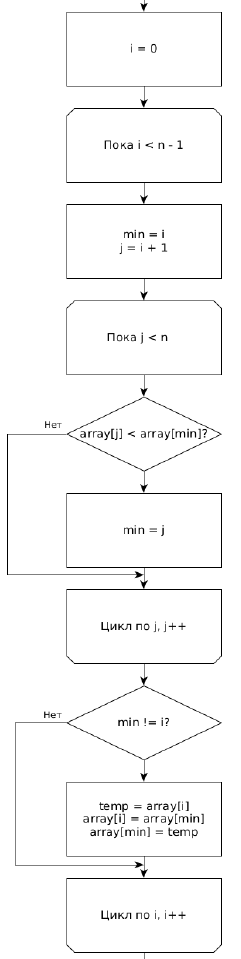
\includegraphics[scale=0.7]{inc/img/selectionfi.png}
\captionsetup{justification=centering}
	\caption{Часть блок-схемы, определяющая $f_{i}$.}
	\label{img:selection:fi}	
\end{center}
\end{figure}
\newpage 

\section*{Вывод}
На основе теоретических данных, полученных из аналитического раздела, были построены схемы рассматриваемых алгоритмов сортировок, оценены их трудоёмкости в лучшем и худшем случаях.

\chapter{Технологическая часть}
\section{Требования к программному обеспечению}
Программное обеспечение принимает на вход массив целочисленных значений.

В результате выполнения программы должен быть получен упорядоченный по возрастанию массив.

\section{Средства реализации программного обеспечения}
При написании программного продукта был использован язык программирования Kotlin \cite{Kotlin}.

Данный выбор обусловлен следующими факторами:
\begin{itemize}
\item Возможность портирования алгоритмов для работы с Android;
\item Возможность часто употреблять выражение "Ко-ко-котлин" или "Котик";
\item Большое количество справочной литературы, связанной с ЯП Java.
\end{itemize}

Для тестирования производительности реализаций алгоритмов использовалась утилита measureTimedValue.

При написании программного продукта использовалась среда разработки IntelliJ IDEA.

Данный выбор обусловлен тем, что язык программирования Kotlin - это разработка компании JetBrains, поставляющей данную среду разработки.

\section{Листинг кода}
В листингах \ref{list:bubbleSort} - \ref{list:selectionSort} предоставлены реализации рассматриваемых алгоритмов.
\begin{lstlisting}[caption=Функция реализации алгоритма сортировки пузырьком,
label={list:bubbleSort}]
fun bubbleSort(arr: IntArray)
{
    var i = 0;
    while (i < arr.size - 1)
    {
        var j = 0;
        while (j < arr.size - 1 - i)
        {
            if (arr[j] > arr[j + 1])
                arr[j + 1] = arr[j].also { arr[j] = arr[j + 1] }
            j++
        }
        i++
    }
}
\end{lstlisting}

\begin{lstlisting}[caption=Функция реализации алгоритма сортировки вставками,
label={list:insertionSort}]
fun insertionSort(arr: IntArray)
{
    var i = 1;
    while (i < arr.size)
    {
        var min = arr[i]
        var j = i;
        while (j > 0 && arr[j - 1] > min)
        {
            arr[j] = arr[j - 1]
            j--
        }
        arr[j] = min
        i++
    }
}
\end{lstlisting}

\begin{lstlisting}[caption=Функция реализации алгоритма сортировки выбором,
label={list:selectionSort}]
fun selectionSort(arr: IntArray)
{
    var i = 0;
    while (i < arr.size - 1)
    {
        var j = i + 1
        var min = i
        while (j < arr.size)
        {
            if (arr[j] < arr[min])
                min = j
            j++
        }
        if (min != i)
            arr[i] = arr[min].also { arr[min] = arr[i] }
        i++
    }
}
\end{lstlisting}

\section{Тестирование программного продукта}
В таблице~\ref{tests} приведены тесты для функций, реализующих алгоритм сортировки пузырьком, вставками и выбором. Тесты пройдены успешно.

\begin{table}[h!]
	\begin{center}
	\caption{\label{tests}Тестирование функций}
		\begin{tabular}{|c|c|c|}
			\hline
			Начальный массив & Ожидаемый результат & Полученный результат \\ 
			\hline
			$[5, 4, 3, 2, 1]$ & $[1, 2, 3, 4, 5]$  & $[1, 2, 3, 4, 5]$\\
			$[0, 0, 0]$  & $[0, 0, 0]$  & $[0, 0, 0]$\\
			$[1, 2, 3]$ & $[1, 2, 3]$ & $[1, 2, 3]$\\
			$[-8, 2, 3, -2]$ & $[-8, -2, 2, 3]$ & $[-8, -2, 2, 3]$\\
			$[]$  & $[]$  & $[]$\\
			\hline
		\end{tabular}
	\end{center}
\end{table}
\section*{Вывод}
Спроектированные алгоритмы сортировок были реализованы и протестированы.

\chapter{Исследовательская часть}

\section{Пример работы программного обеспечения}
Ниже на рисунках \ref{img:exampleOut1}- \ref{img:exampleOut2} предоставлены примеры работы каждого из алгоритмов на введённых пользователем данных.

\begin{figure}
\begin{center}
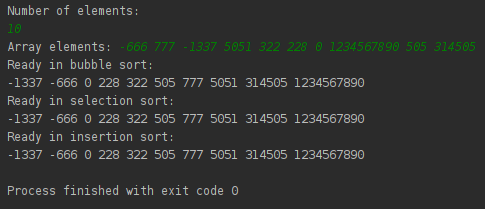
\includegraphics[scale=1]{inc/img/exampleOutput.png}
\captionsetup{justification=centering}
	\caption{Пример работы ПО.}
	\label{img:exampleOut1}	
\end{center}
\end{figure}

\begin{figure}
\begin{center}
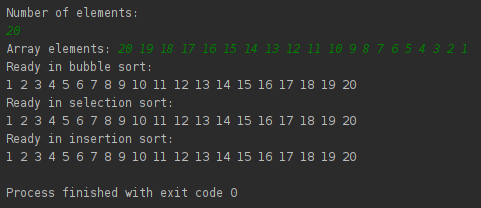
\includegraphics[scale=1]{inc/img/exampleOutput1.png}
\captionsetup{justification=centering}
	\caption{Пример работы ПО.}
	\label{img:exampleOut2}	
\end{center}
\end{figure}

\newpage

\section{Технические характеристики}
Технические характеристики ЭВМ, на котором выполнялись исследования:
\begin{itemize}
\item ОС: Manjaro Linux 20.1.1 Mikah
\item Оперативная память: 16 Гб
\item Процессор: Intel Core i7-10510U
\end{itemize}


При проведении замеров времени ноутбук был подключен к сети электропитания.

\section{Время выполнения алгоритмов}
Алгоритмы тестировались на данных, сгенерированных случайным образом один раз.

Результаты замеров времени приведены в таблицах \ref{time1} - \ref{time3}. На рисунках \ref{timeRes1} и \ref{timeRes3} приведены графики зависимостей времени работы алгоритмов от количества элементов в случаях передачи упорядоченного, неупорядоченного и упорядоченного в обратном порядке массива. В таблице СП - Сортировка Пузырьком, СВст - Сортировка Вставками, СВыб - Сортировка выбором.

\newpage
\begin{table}[h]
	\begin{center}
		\caption{\label{time1} Замеры времени для упорядоченных массивов}
		\begin{tabular}{|c c c c|} 
 			\hline
			Размер массива & СП & СВст & СВыб \\ [0.5ex] 
 			\hline\hline
 			100 & 1818544 & 1630961 & 1826308\\
 			\hline
 			200 & 2182084 & 1647635 & 2144446 \\
 			\hline
			300 & 2836575 & 1640207 & 2530081\\
			\hline
			400 & 3666706 & 1640022 & 2924786\\
			\hline
			500 & 4561938 & 1645407 & 3594866\\
			\hline
			1000 & 12282615 & 1654109 & 8634889\\
			\hline
			1500 & 25296835 & 1662390 & 17374004\\
			\hline
			2000 & 43069012 & 1700609 & 29104145\\
			\hline
			3000 & 91881622 & 1810398 & 61997393\\
			\hline
			4000 & 165458964 & 1823571 & 105764286\\
			\hline
			5000 & 248940636 & 1766772 & 164210924\\
			\hline
			\end{tabular}
	\end{center}
\end{table}

\newpage

\begin{table}[h]
	\begin{center}
		\caption{\label{time2} Замеры времени для упорядоченных в обратном порядке массивов}
		\begin{tabular}{|c c c c|} 
 			\hline
			Размер массива & СП & СВст & СВыб \\ [0.5ex] 
 			\hline\hline
 			100 & 1902381 & 1770645 & 1712426\\
 			\hline
 			200 & 2690147 & 2035881 & 1948340\\
 			\hline
			300 & 3973067 & 2809635 & 2299634\\
			\hline
			400 & 6108805 & 3078558 & 2837866\\
			\hline
			500 & 8344909 & 3876786 & 3483199\\
			\hline
			1000 & 28119897 & 10741734 & 9179446\\
			\hline
			1500 & 59508253 & 21659401 & 17961391\\
			\hline
			2000 & 102249552 & 37367527 & 30242327\\
			\hline
			3000 & 218854972 & 78513340 & 65218978\\
			\hline
			4000 & 379629421 & 131840967 & 114500414\\
			\hline
			5000 & 592686305 & 197947307	& 173933001\\
			\hline
			\end{tabular}
	\end{center}
\end{table}

\newpage

\begin{table}[h]
	\begin{center}
		\caption{\label{time3} Замеры времени для неупорядоченных массивов}
		\begin{tabular}{|c c c c|} 
 			\hline
			Размер массива & СП & СВст & СВыб \\ [0.5ex] 
 			\hline\hline
 			100 & 1592950 & 1498909 & 1460379\\
 			\hline
 			200 & 2200640 & 1562519 & 1680307\\
 			\hline
			300 & 3280409 & 1808384 & 2038358\\
			\hline
			400 & 4728961 & 2184299 & 2558087\\
			\hline
			500 & 6573267 & 2566161 & 3166091\\
			\hline
			1000 & 21195842 & 5769483 & 8411547\\
			\hline
			1500 & 45146080 & 11233626 & 17161009\\
			\hline
			2000 & 79173129 & 18556919 & 28673064\\
			\hline
			3000 & 166840980 & 38942468 & 64444295\\
			\hline
			4000 & 280142359 & 66181509 & 102043152\\
			\hline
			5000 & 449032194 & 99391239 	& 172713187\\
			\hline
			\end{tabular}
	\end{center}
\end{table}

\begin{figure}[h]
\begin{center}
	\begin{tikzpicture}

\begin{axis}[
  		  	axis lines = left,
  		  	xlabel = размер,
  		  	ylabel = {время, нс},
			legend pos=north west,
			ymajorgrids=true
		] 
		\addplot[color=orange] table[x index=0, y index=1] {SBSorted.dat};
		\addplot[color=blue, mark=square] table[x index=0, y index=1] {SISorted.dat};
		\addplot[color=green, mark=square] table[x index=0, y index=1] {SSSorted.dat};

		\addlegendentry{СП}
		\addlegendentry{СВст}
		\addlegendentry{СВыб}
		\end{axis}
	\end{tikzpicture}
	\captionsetup{justification=centering}
	\caption{Зависимость времени работы от размера отсортированных массивов}
	\label{timeRes1}
	\end{center}
\end{figure}

\newpage

\begin{figure}[h]
\begin{center}
	\begin{tikzpicture}

\begin{axis}[
  		  	axis lines = left,
  		  	xlabel = размер,
  		  	ylabel = {время, нс},
			legend pos=north west,
			ymajorgrids=true
		] 
		\addplot[color=orange] table[x index=0, y index=1] {SBSortedReverse.dat};
		\addplot[color=blue, mark=square] table[x index=0, y index=1] {SISortedReverse.dat};
		\addplot[color=green, mark=square] table[x index=0, y index=1] {SSSortedReverse.dat};

		\addlegendentry{СП}
		\addlegendentry{СВст}
		\addlegendentry{СВыб}
		\end{axis}
	\end{tikzpicture}
	\captionsetup{justification=centering}
	\caption{Зависимость времени работы от размера отсортированных в обратном порядке массивов}
	\label{timeRes2}
	\end{center}
\end{figure}

\begin{figure}[h]
\begin{center}
	\begin{tikzpicture}
	
\begin{axis}[
  		  	axis lines = left,
  		  	xlabel = размер,
  		  	ylabel = {время, нс},
			legend pos=north west,
			ymajorgrids=true
		] 
		\addplot[color=orange] table[x index=0, y index=1] {SBUnsorted.dat};
		\addplot[color=blue, mark=square] table[x index=0, y index=1] {SIUnsorted.dat};
		\addplot[color=green, mark=square] table[x index=0, y index=1] {SSUnsorted.dat};

		\addlegendentry{СП}
		\addlegendentry{СВст}
		\addlegendentry{СВыб}
		\end{axis}
	\end{tikzpicture}
	\captionsetup{justification=centering}
	\caption{Зависимость времени работы от размера массивов, заданных случайным образом}
	\label{timeRes3}
	\end{center}
\end{figure}

\newpage

\section*{Вывод}
При сравнении результатов замеров по времени видно, что выводы в каждом из случаев неоднозначны.

В случае уже отсортированных массивов, однозначно лучше всех показывает себя сортировка вставками. Связано это с особенностями реализации алгоритма, зависимость в текущих обстоятельствах будет, теоретически, линейной. Поэтому целесообразно указать на факт того, что сортировка пузырьком уже на 3000 элементов будет работать медленнее, чем сортировка выбором на  $\approx 50.8 \%$, при этом с увеличением количества элементов массива, это значение будет расти.

В случае упорядоченного в обратном порядке массива, что можно назвать наихудшим случаем, лучше всех показывает себя сортировка выбором. При этом, разница между временем работы сортировки выбором и сортировки вставками на 4000 элементов массива будет равна $\approx 15\%$. Но наибольшая разница, которая заключается между временем работы сортировки выбором и сортировки пузырьком на 5000 элементов: $\approx 340\%$.

Ситуация несколько изменится при рассмотрении скорости работы алгоритмов на массивах чисел, сгенерированных случайно. Здесь можно будет увидеть преобладание алгоритма сортировки выбором над алгоритмом сортировки вставками. На значениях величины массива, равных 4000, разница в скорости обработки будет составлять $\approx 65\%$. Наибольшая выявленная разница в скорости работы алгоритма вставками и алгоритма сортировки пузырьком будет составлять $\approx 260\%$.

Таким образом, учитывая ситуацию каждого из случаев, можно сказать, что в описанных ситуациях оптимальный вариант - использование сортировки вставками.

\chapter*{Заключение}
\addcontentsline{toc}{chapter}{Заключение}
В ходе выполнения лабораторной работы была достигнута цель и выполнены следующие задачи:
\begin{enumerate}
\item были реализованы алгоритмы сортировки пузырьком, вставками и выбором;
\item был проведён сравнительный анализа трудоёмкости алгоритмов на основе теоретических расчетов и выбранной модели вычислений;
\item был проведён сравнительный анализ алгоритмов на основе экспериментальных данных;
\item был подготовлен отчёт по лабораторной работе;
\item были получены практические навыки реализации алгоритмов на ЯП Kotlin.
\end{enumerate}

Исследования показали, что хуже всего себя показала реализация алгоритма сортировки пузырьком.

При сортировке уже отсортированного массива "пузырёк" будет работать на $\approx 66\%$ медленнее при сортировке 5000 элементов, чем алгоритм сортировки выбором. Но наилучшим вариантом в данном случае будет выбор алгоритма сортировки вставками, так как возрастание скорости его работы в данном случае линейно.

В случае отсортированного в обратном порядке массива лучше всего себя показывает сортировка вставками, она в $\approx 1.38$ раз быстрее алгоритма сортировки выбором. Наибольшая разница, которая заключается между временем работы сортировки выбором и сортировки пузырьком на 5000 элементов: $\approx 340\%$.

Но в случае неупорядоченных массивов лучше всего себя показывает сортировка вставками, она в $\approx 1.74$ раза быстрее, чем сортировка выбором уже на 5000 элементов. Наибольшая выявленная разница в скорости работы алгоритма вставками и алгоритма сортировки пузырьком будет составлять $\approx 260\%$

\addcontentsline{toc}{chapter}{Литература}
\bibliographystyle{utf8gost705u}  % стилевой файл для оформления по ГОСТу
\bibliography{biblio.bib}          % имя библиографической базы (bib-файла)


\end{document} 
